\documentclass[times, utf8, seminar, numeric]{fer}
\usepackage{booktabs}
\usepackage{url}
\usepackage{listings}
\usepackage{color}

\lstset{
language=C,                % choose the language of the code
basicstyle=\footnotesize,       % the size of the fonts that are used for the code
numbers=left,                   % where to put the line-numbers
numberstyle=\footnotesize,      % the size of the fonts that are used for the line-numbers
stepnumber=1,                   % the step between two line-numbers. If it is 1 each line will be numbered
numbersep=5pt,                  % how far the line-numbers are from the code
backgroundcolor=\color{white},  % choose the background color. You must add \usepackage{color}
showspaces=false,               % show spaces adding particular underscores
showstringspaces=false,         % underline spaces within strings
showtabs=false,                 % show tabs within strings adding particular underscores
frame=tb,           % adds a frame around the code
tabsize=2,          % sets default tabsize to 2 spaces
captionpos=b,           % sets the caption-position to bottom
breaklines=false,        % sets automatic line breaking
breakatwhitespace=false,    % sets if automatic breaks should only happen at whitespace
escapeinside={\%*}{*)}          % if you want to add a comment within your code
}


\begin{document}

\renewcommand{\figurename}{Slika}
\renewcommand{\tablename}{Tablica}
\renewcommand{\lstlistingname}{Programski odsječak}
\newtheorem{lema}{Lema}

% TODO: Navedite naslov rada.
\title{Izgradnja sufiksnog stabla - Ukkonenov algoritam}

% TODO: Navedite vaše ime i prezime.
\author{Frane Kurtović i Matija Šantl}

% TODO: Navedite ime i prezime mentora.
\voditelj{doc. dr. sc. Mirjana Domazet-Lošo}

\maketitle

\tableofcontents

\chapter{Uvod}
Sufiksno stablo \engl{suffix tree} je stablasta struktura podataka koja sadrži sve sufikse nekog niza znakova \cite{ukkonen}. Sufiksno stablo na elegantan način rješava problem pretraživanja podniza u nizu, precizinije, podniz je moguće pronaći u vremenu proporcionalnom duljini podniza \cite{mile}. Jedna takva primjena je pronalazak najduljeg zajedničkog podniza dvaju nizova u vremenu porporcionalnom zbroju njihovih duljina \cite{gusfield}.
	
	Sufiksno stablo može biti izgrađeno u vremenu linearno ovisnom o duljini ulaznog niza. Današnji standard je \textit{Ukkonenov} algoritam iz 1995. godine. To je prvi \textit{on-line} algoritam za izgradnju sufiksnog stabla \cite{mile}.
		
\section{Osnovni pojmovi}
	Neka je $T = t_1 t_2 ... t_n$ niz znakova nad abecedom $\Sigma$. Svaki niz znakova $x$ takav da je $T=u x v$ za neke (moguće i prazne) nizove $u$ i $v$ nazivamo podnizom od $T$.

U ovom tekstu korištene su sljedeće oznake:
\begin{itemize}
	\item ulazni niz znakova je označen s $T$,
	\item duljina ulaznog niza znakova $T$ je označena s $n$
	\item \textit{prefiks} niza $T$ je podniz $T[1, i]$ te je označen s $T^i$, $1 \le i \le n$
	\item \textit{sufiks} niza $T$ je podniz $T[i, n]$ te je označen s $T_i$, $1 \le i \le n + 1$
	\item posebno, $T_{n+1}$ je prazan sufiks, $T_{n+1} = \epsilon$
	\item skup svih sufiksa niza znakova $T$ je označen s $\sigma(T)$
	\item stoblo sufiksa \engl{suffix trie} je stoblo koje predstavlja $\sigma(T)$
\end{itemize}

\chapter{Opis algoritma}
	\textit{Ukkonenov} algoritam se može predstaviti kao linearna verzija algoritma za sufiksna stobla koji je kvadratne složenosti. Taj je algoritam opisan u poglavlju 2.1. Jednom transparentnom promjenom, koja je opisana u poglavlju 2.3, dolazimo do algoritma linearne složenosti, poznatijeg pod nazivom \textit{Ukkonenov} algoritam za izgradju sufiksnog stabla u linearnom vremenu.

\section{Izgradnja sufiksnog stobla}
	Formalno, sufiksno se stoblo može definirati kao petorka $STrie(T) = (Q \cup {\perp}, root, F, g, f)$, i možemo reći da je takvo stoblo prošireni deterministički konačni automat koji ima stablolik graf prijelaza koji predstavljaju stoblo $\sigma(T)$ koje je prošireno sa tzv. funkcijom sufiksa \engl{suffix function} $f$ i pomoćnim stanjem $\perp$. Skup $Q$ od stanja $STrie(T)$ se može staviti u jedan-naprema-jedan vezu s podnizovima niza $T$. Stanje koje odgovara podnizu $x$ oznacavamo s $\overline{x}$.
	
	Početno stanje $root$ odgovara praznom nizu $\epsilon$, a skup F završnom skupu stanja  $\sigma(T)$. Funkcija prijelaza $g$ je definirana kao $g(\overline{x}, a) = \overline{y}$ za sve $\overline{x}$, $\overline{y}$ u $Q$ tako da $y = x a$ pri čemu je $a \in \Sigma$.
	
	Funkcija sufiksa $f$ je definirana za svako stanje $\overline{x} \in Q$ na sljedeći način. Neka je $\overline{x} \ne root$. Onda $x = ay$ za neki $a \in \Sigma$, i $f(\overline{x}) = \overline{y}$. Dodatno, $f(root) = \perp$.
	
	Pomoćno stanje $\perp$ nam omogućava pisanje algoritama u nastavcima tako da se izbjegne eksplicitna razlika između praznih i ne-praznim sufiksa. Stanje $\perp$ je spojeno na stoblo s $g(\perp, a) = root$ za svaki $a \in \Sigma$. 
	
	U skladu s \cite{ukkonen}, funkciju sufiksa $f(r)$ nazivamo sufiksnom vezom \engl{suffix link} stanja $r$. 
	
	On-line izgradnja sufiksnog stobla $STrie(T)$ radi se prolaskom niz $T$ s lijeva na desno. Kao međurezultat izgradnje dobijamo $STrie(T^i)$ za $i=0, 1, ..., n$. 
	Ključna primjedba koja opisuje kako se $STrie(T^i)$ dobija iz $STrie(T^{i-1})$ je da se sufiksi od $T^i$ mogu dobiti dodavanjem $t_i$ na kraj svakog sufiksa od $T^{i-1}$ i dodavanjam praznog sufiksa, tj. $$ \sigma(T^i) = \sigma(T^{i-1}) \cup {\epsilon}$$
	
	Prema definiciji, $STrie(T^{i-1})$ prihvaća $\sigma{T^{i-1}}$. Kako bismo dobili da prihvaća i $\sigma{T^{i}}$, moramo proučiti skup završnih stanja $F_{i-1}$ od $STrie(T^{i-1})$. Ako $r \in F_{i-1}$ još nije $t_{i}$-prijelaz , prijelaz od $r$ prema novom stanju se dodaje. Stanja u koja vode neki stari ili novi $t_{i}$-prijelazi iz nekog stanja $F_{i-1}$ zajedno sa stanjem $root$ čine završna stanja $F_i$ od $STrie{T^{i}}$.
	
	Stanja $r \in F_{i-1}$ koja dobe nove prijelaze mogu se pronaći koristeći sufiksne veze na sljedeći način. Definicija sufiksne funkcije implicira da je $r \in F_{i-1}$ ako i samo ako $r = f^{j} (\overline{t_1 ... t_{i-1}}) $ za neki $0 \le j \le i-1$. Zbog toga su sva stanja u $F_{i-1}$ na putu sufiksne veze koja počinje na najdubljem stanju $\overline{t_1 .. t_{i-1}}$ od $STrie(T^{i-1})$ i završava na $\perp$. Taj se put zove granični put \engl{boundary path} od $STrie(T^{i-1})$.
	
	Ako stanje $\overline{z}$ na graničnom putu još nema prijelaz na $t_i$, novo stanje $\overline{z t_i}$ i novi prijelaz $g(\overline{z}, t_i) = \overline{z t_i}$ se dodaje. Time osvježavamo funkciju prijelaza, $g$. Funkciju sufiksa, $f$, osvježavamo tako da nova stanja $\overline{z t_i}$ povezujemo s novim sufiksnim vezama koje čine put koji počinje u stanju $\overline{t_1 t_2 .. t_i}$, tj. granični put od $STrie(T^i)$. 
	
	Prolazak preko $F_{i-1}$ na graničnom putu se može odmah zaustaviti kada je pronađeno prvo stanje $\overline{z}$ takvo da stanje $\overline{z t_i}$ (a time i prijelaz $g(\overline{z}, t_i) = \overline{z t_i}$) već postoji. Neka je $\overline{z t_i}$ stanje. Onda $STrie(T^{i-1})$ mora sadržavati stanje $\overline{z\rq{} t_i}$ i prijelaz $g(\overline{z\rq{}}, t_i) = \overline{z\rq{} t_i}$ za svaki $\overline{z\rq{}} = f^j(\overline{z})$, $j \ge 1$. Drugim riječima, ako je $z t_i$ podniz od $T^{i-1}$ onda je svaki sufiks od $z t_i$ podniz od $T^{i-1}$. Stanje $\overline{z}$ će uvijek postojati jer je stanje $\perp$ zadnje stanje na graničnom putu i stanje $\perp$ ima definiran prijelaz za svaki mogući $t_i$.
	
	Kada je takav obilazak završio, stvorit ćemo novo stanje za svaku sufiks vezu koju smo pregledali tijekom obilaska. To implicira da će cijeli postupak trajati ovisno o veličini dobivenog automata.
	
	U nastavku je prikazan algoritam za izgradnju stobla $STrie{T^i}$ iz $STrie(T^{i-1})$, pri čemu je \textit{top} zapravo stanje $\overline{t_1 ... t_{i-1}}$;
	
\begin{lstlisting}[caption=Izgradnja $STrie(T^i)$ iz $STrie(T^{i-1})$, label=algo1]
r = top;
dok je g(r, t[i]) nedefinirano
	stvori novo stanje r` i novi prijelaz g(r, t[i]) = r`;
	ako je r != top onda: stvori novu sufiksnu vezu f(oldr`) = r`;
	oldr` = r`;
	r = f(r);
stvori novu sufiksnu vezu f(oldr`) = g(r, t`);
top = g(top, t[i])
\end{lstlisting}
	
	Počevši od $STrie(\epsilon)$, koje se sastoji samo od stanja $root$, $\perp$ i veza između njih, ponavljanjem procedure \ref{algo1} za $t_i = t_1,t_2,...t_n$ dobijamo $STrie(T)$. Algoritam je optimalan u smislu da je vremenska složenost proporcionalna konačnom rezultatu, $STrie(T)$, a to je proporcionalno s $|Q|$, tj. brojem različitih podnizova od $T$. Međutim, to može dovesti do kvadratne složenosti u $|T|$, ako je npr. $T=a^n b^n$.

\section{Sufiksno stablo}
	Sufiksno stablo $STree(T)$ nad nizom $T$ je struktura podataka koja predstavlja $STrie(T)$ u prostoru koji je linearan s duljinom $|T|$ niza $T$ \cite{ukkonen}. To se postiže tako da ne koristimo sva, već samo podskup stanja $Q\rq{} \cup {\perp}$ svih stanja od $STrie(T)$. Ta stanja nazivamo eksplictna stanja \engl{explicit states}. Skup $Q\rq{}$ se sastoji od granajućih stanja \engl{branching state}, stanja koja imaju barem dva prijelaza, i listova \engl{leaves}, stanja koja nemaju prijelaza. Po definiciji, stanje $root$ je uključeno u granajuća stanja. Sva preostala stanja $STrie(T)$ zovemo implicitna stanja \engl{implicit states} sufiksnog stabla $STree(T)$.
	
	Niz znakova $w$ koji se nalazi na putu u stoblu $STrie(T)$ između dva eksplicitna stanja $s$ i $r$ je u stablu $STree(T)$ predstavljen kao generalizirani prijelaz $g\rq{}(s, w) = r$. Kako bi uštedjeli na prostoru, niz znakova $w$ je zapravo prikazan uređenim parom pokazivača $(k, p)$ na $T$ takvih da je $w = t_k ... t_p$. Zbog toga, generalizirani prijelaz ima oblik $g\rq{}(s,(k, p)) = r$.
	
	Prijelaz $g\rq{}(s, (k, p)) = r$ nazivamo \textit{a-prijelaz} ako je $t_k = a$. Svako stanje $s$ može imati najviše jedan \textit{a-prijelaz} za svaki $a \in \Sigma$.
	
	Prijelazi $g(\perp, a) = root$ su prikazani na sličan način. Neka je $\Sigma = {a_1, a_2, ..., a_m}$. Onda je prijelaz $g(\perp, a_j) = root$ prikazan kao $g(\perp, (-j, -j)) = root$ za $j = 1, ... , m$.
	
	Zbog toga, sufiksno stablo $STree(T)$ ima dvije komponente: niz znakova $T$ i samo stablo. Ono je linearne veličine u $|T|$ jer skup $Q\rq{}$ ima najviše $|T|$ listova (postoji najviše jedan list za svaki ne-prazni sufiks) i zbog toga skup $Q\rq{}$ mora sadržavati najviše $|T| - 1$ granajućih stanja. Može postojati najviše $2|T| - 2$ prijelaza između stanja u skupu $Q\rq{}$, gdje svaki prijelaz zauzima konstatan prostor zbog korištenja pokazivača.
	
	Stablo se dodatno proširuje sa sufiksnom funkcijom $f\rq{}$, koja je sada definirana za sva granajuća stanja $\overline{x} \ne root$ kao $f\rq{}(\overline{x}) = \overline{y}$ gdje je $y$ takvo granajuće stanje da je $x = ay$ za neki $a \in \Sigma$, i $f\rq{}(root) = \perp$. 
	
	Formalno, sufiksno stablo možemo predstaviti uređenom četvorkom kao $STree(T) = (Q\rq{} \cup {\perp}, root, g\rq{}, f\rq{})$.
	
	Na neko implicitno ili eksplicitno stanje sufiksnog stabla $r$ se referenicramo pomoću uređenog para $s, w$ gdje je $s$ neko eksplicitno stanje koje prethodi stanju $r$ a $w$ je niz znakova koje posjećujemo na putu od $s$ prema $r$ u odgovarajućem sufiksnom stoblu. Referentni par \engl{reference pair} se naziva kanonskim \engl{canonical} ako je stanje $s$ najbliži predak stanja $r$ (i prema toma niz $w$ je najkraći mogući). Za takvo eksplicitno stanje $r$, kanonski referentni par je $(r, \epsilon)$, tj. budući da koristimo pokazivače, taj par poprima oblik $(r, (p+1, p))$ pri čemu je $w = t_k ... t_p$.
	
	Eksplicitna završrna stanja dobivamo dodavanjem oznake kraja na $T$ koja se ne pojavljuje nigdje u $T$.

\section{On-line izgradnja sufiksnog stabla}

	Neka su $s_1 = \overline{t_1 ... t_{i-1}}$, $s_2, s_3, ..., s_i = root$, $s_{i+1} = \perp$ stanja sufiksnog stobla $STrie(T^{i-1})$ koja se nalaze na graničnom putu. Neka je $j$ najmanji indeks takav da $s_j$ nije list, i neka je $j\rq{}$ najmanji indeks takav da $s_{j\rq{}}$ ima $t_i$-prijelaz.
	
\begin{lema}
Algoritam \ref{algo1} dodaje u $STrie(T^{i-1})$ jedan $t_i$-prijelaz za svako stanje $s_h$, $1 \le h \le j\rq{}$ takvo da je $1 \le h \le j$, novi prijelaz proširuje postojeće grane stobla koje završavaju na listu $s_h$, a za $j \le h \le j\rq{}$, stvara nove prijelaze koji se granaju iz $s_h$.
\end{lema}

	Stanje $s_j$ zovemo aktivnom točkom \engl{active point} a stanje $s_{j\rq{}}$ završnom točkom \engl{end point} sufiksnog stobla $STrie(T^{i-1})$. Ta stanja postoje kao eksplicitna ili implicitna i u sufiksnom stablu $STree(T^{i-1})$. 
	
	Prema \textit{Lema 1}, algoritam \ref{algo1} dodaje dvije skupine $t_i$-prijelaza u $STrie(T^{i-1})$.

\begin{enumerate}
	\item Stanja na graničnom putu prije aktivne točke $s_j$ dobijaju prijelaz. Ta stanja su listovi pa zbog toga svaki prijelaz mora proširiti postojeće grane sufiksnog stobla.
	\item Stanja nakon aktivne točke $s_j$ pa sve do završne točke $s_{j\rq{}}$ (ne uključujući) dobijaju novi prijelaz, a budući da ta stanja nisu listovi, ti prijelazi moraju započeti novu granu.
\end{enumerate}

	Prva skupina prijelaza se može implementirati kao osvježavanje desnog pokazivača od svakog prijelaza koji predstavlja granu. Neka je $g\rq{}(s, (k, i-1)) = r$ jedan takav prijelaz. Desni pokazivač mora pokazivati na zadnju poziciju, i-1, od $T^{i-1}$. Zbog toga što je stanje $r$ list, svaki put koji vodi do $r$ mora biti jedan sufiks od $T^{i-1}$ koji se ne pojavljuje nigdje drugdje unutar $T^{i-1}$. Tada osvježeni prijelaz mora biti $g\rq{}(s, (k, i)) = r$. Time se uopće ne mijenjaju stanje $r$ i $s$ već samo niz znakova koji nastaje obilaskom puta. Kako bi osvježavanje svakog takvog stanja zasebno bilo vremenski preskupo, koristi se sljedeći trik.

	Svaki prijelaz stable $STrer(T^{i-1})$ koji vodi ka listu se zove otvoreni prijelaz \engl{opem transition}. Takav je prijelaz oblika $g\rq{}(s, (k, i-1)) = r$. Budući da desni pokazivač mora pokazivati na zadnju poziciju $i-1$ od $T^{i-1}$, nije nužno da desni pokazivač ima ispravnu vrijednost, već se umjesto toga otvoreni prijelazi mogu predstaviti kao $g\rq{}(s, (k, \infty)) = r$ gdje $\infty$ označava da otvoreni prijelaz može \lq\lq{}rasti\rq\rq{}. $g\rq{}(s, (k, \infty)) = r$ zapravo predstavlja granu bilo koje duljine između stanja $s$ i imaginarnog stanja $r$ koje je u \lq\lq{}beskonačnosti\rq\rq{}. Zbog toga nije potrebno eksplicitno osvježavanje desnog pokazivača kada se umeće $t_i$ u granu. Oznake $\infty$ se mogu zamijeniti s $n = |T|$ nakon što smo završili izgradnju stabla $STree(T)$.
	
	Druga skupina prijelaza stvara sasvim nove grane koje počinju u stanjima $s_h$, $j \le h \le h\rq{}$. Traženje takvih stanja $s_h$ zahtjeva malo pažnje budući da ne moraju nužno biti eksplicitna u tom trenutku. Takva ćemo stanja nalaziti na graničnom putu stabla $STree(T^{i-1})$ koristeći referentne parove i sufiksne veze.
	
	Neka je $h = j$ i neka je $(s, w)$ kanonski referentni par za $s_h$ za recimo aktivnu točku. Kako je $s_h$ na graničnom putu stobla $STrie(T^{i-1})$, $w$ mora biti sufiks od $T^{i-1}$. Zbog toga je $(s, w) = (s, (k, i - 1))$ za neki $k \le i$.
	
	Želimo li kreirati novu granu koja počinje u stanju na koje se referenciramo s $(s, (k, i-1))$, moramo najprije provjeriti da li se možda $(s, (k, i- 1))$ već referencira na stanje $s_{j\rq{}}$. Ako se referencira onda smo gotovi. Inače moramo stvoriti novu granu. Stanje na koje se referenciramo s $(s, (k, i-1))$, $s_h$ mora biti eksplicitno do sad. Ako stanje $s_h$ nije eksplicitno, ono se stvara dijeljenjem prijelaza koje sadrži odgovarajuće implicitno stanje. Tek onda se stvara $t_i$-prijelaz iz stanja $s_h$. Taj prijelaz mora biti otvoreni prijelaz, tj. $g\rq{}(s_h, (i, \infty)) = s_{h\rq{}}$ pri čemu je $s_{h\rq{}}$ novi list. K tome, dodaje sufiksna veza $f\rq{}(s_h)$ ako je stanje $s_h$ nastalo dijeljenjem prijelaza.
	
	Nako toga se izgradnja pomiče na $s_{h+1}$. Budući  da je referentni par za $s_h$ bio $(s, (k, i-1))$, kanonski referentni par za $s_{h+1}$ će biti $canonize(f\rq{}(s), (k, i-1))$ pri čemu $canonize$ stvara referentni par kanonskim tako da osvježi stanje i lijevi pokazivač. Gornje navedene operacije se tada ponavljaju za $s_{h+1}$ pa sve dok se pronađe završna točka $s_{j\rq{}}$.
	
	Na taj način radi funkcija $update$ koja je prikazana u programskom odsječku \ref{update}. Ta funkcija pretvara stablo $STree(T^{i-1})$ u $STree(T^i)$ umetanjem $t_i$-prijelaza iz druge skupine. Funkcija koristi pomoćne funkcije $canonize$ koje je spomenuta gore, te $test-and-split$ koja provjerava da li se dani referentni par referencira na završnu točku. Ako se ne referencira na završnu točku tada funkcija $test-and-split$ stvara i vraća novo eksplicitno stanje za dani referentni par ako se taj referentni par već ne referancira na eksplicitno stanje. Funkcija $update$ vraća referentni par za završnu točku $s_{j\rq{}}$.
	
	
\begin{lstlisting}[caption=Funkcija $update$, label=update]
funkcija update(s, (k, i)):
	// (s, (k, i - 1)) je kanonski referentni par za aktivnu tocku
	stari_root = root
	(zavrsna_tocka, r) = test_and_split(s, (k, i-1), t[i])
	
	dok je zavrsna_tocka = False
		stvori novi prijelaz g`(r, (i, INF)) = r` 
		ako je stari_root != root onda
			stvori novu sufiksnu vezu f`(stari_root) = r
		stari_root  = r
		(s, k) = canonize(f`(s), (k, i-1))
		(zavrsna_tocka, r) = test_and_split(s, (k, i- 1), t[i])
		
	ako je stari_root != root onda
		stvori novu sufiksnu vezu f`(stari_root) = s

	vrati (s, k)
\end{lstlisting}

	Funkcija $test-and-split$ provjerava da li je stanje s kanonskim referentnim parom $(s, (k, p))$ završna točka, tj. da li bi to stanje u stoblu $STrie(T^{i-1})$ imalo $t_i$-prijelaz. Simbol $t_i$ je dan kao ulazni parametar $t$. Ako $(s, (k, p))$ nije završna točka, stanje (s, (k, p)) se napravi eksplicitnim ako još nije tako da se podijeli prijelaz. 

\begin{lstlisting}[caption=Funkcija $test-and-split$, label=testandsplit]
funkcija test-and-split(s, (k, p), t):
	ako je k <= p onda
		neka je g`(s, (k`, p`)) = s` t[k]-prijelaz iz s;
		ako je t = t[k` + p - k _ 1] onda
			vrati (True, s)
		inace
			zamijeni gornji t[k]-prijelaz s prijelazima
				g`(s, (k`, k` + p - k)) = r
				g`(r, (k` + p - k + 1, p`)) = s`
				pri cemu je r novo stanje
				vrati (False, r)
	inace
		ako ne postoji t-prijelaz iz s
			vrati (False, s)
		inace
			vrati (True, s)
\end{lstlisting}

	Odgovor na pitanje da li je neko stanje završna točka može se naći u konstantnom vremenu promatrajući pritom samo jedan prijelaz is $s$.
	
	Funkcija $canonize$ za dani referentni par $(s, (k, p))$ za neko stanje $r$, nalazi i vraća stanje $s\rq{}$ i lijevi pokazivač $k\rq{}$ takvi da $(s\rq{}, (k\rq{}, p))$ bude referentni par za stanje $r$. Stanje $s\rq{}$ je najbliži eksplicitni predak stanja $r$ (ili stanje $r$ ako je ono eksplicitno). Zbog toga niz znakova koji vode iz $s\rq{}$ u $r$ mora biti sufiks niza $t_k ... t_p$ koj vodi iz $s$ u $r$. Iz tog se razloga desni pokazivač ne mijenja, dok lijevi može postati $k\rq{}$, $k\rq{} \ge k$.
	
\begin{lstlisting}[caption=Funkcija $canonize$, label=canonize]
funkcija canonize(s, (k, p)):
	ako je p < k onda
		vrati (s, k)
	inace
		pronadi t[k]-prijelaz g`(s, (k`, p`)) = s` iz s
		dok je p` - k` <= p - k
			k = k + p` - k` + 1
			s = s`
			ako je k <= p onda
				nadi t[k]-prijelaz g`(s, (k`, p`)) = s` iz s
				
		vrati (s, k)
\end{lstlisting}

	Kako bi se omogućila daljnja konstrukcija stabla za simbol $t_{i+1}$, mora se pronaći aktivna točka stabla $STree(T^i)$. Stanje $s_j$ je aktivna točka stabla $STree(T^{i-1})$ ako i samo ako je $s_j = \overline{t_j ... t_{i-1}}$ pri čemu je $t_j ... t_{i-1}$ najdulji sufiks od $T^{i-1}$ koji se pojavljuje barem dva puta u $T^{i-1}$. Stanje $s_{j\rq{}}$ je završna točka stabla $STree(T^{i-1})$ ako i samo ako je $s_{j\rq{}} = \overline{t_{j\rq{} ... t_{i-1}}}$ gdje je $t_{j\rq{} ... t_{i-1}}$ najdulji sufiks od $T^{i-1}$ takav da je $t_{j\rq{} ... t_{i-1}} t_i$ podniz od $T^{i-1}$. To znači da ako je $s_{j\rq{}}$ završna točka stabla $STree(T^{i-1})$ onda je $t_{j\rq{} ... t_{i-1}} t_i$ najdulji sufiks od $T^i$ koji se pojavljuje barem dvaput u $T^i$, tj., stanje $g(s_{j\rq{}}, t_i)$ je aktivna točka stabla $STree(T^i)$.
			
\begin{lema}
Neka je $(s, (k, i-1))$ referentni par završne točke $s_j\rq{}$ stabla $STree(T^{i-1})$. Onda je (s, (k, i)) referentni par aktivne točke stabla $STree(T^i)$.
\end{lema}
			
\begin{lstlisting}[caption=Konstrukcija sufiksnog stabla, label=construct]
stvori stanja root i start
za j = 1 do m
	stvori prijelaz g`(, (-j, -j)) = root
stvori sufiksnu vezu f`(root) = start

s = root, k = 1, i = 0
dok t[i+1] nije zavrsni znak
	i = i + 1
	(s, k) = update(s, (k, i))
	(s, k) = canonize(s, (k, i))
\end{lstlisting}

Programski odsječak \ref{construct} konstruira sufiksno stablo $STree(T)$ za ulazni niz znakova $T = t_1 .. t_n$ on-line u vremenskoj složenosti $O(n)$.
						
\chapter{Prikaz rada algoritma}
Izgradnja sufiksnog stabla se odvija redom, dodavajući svaki put novi znak u stablo. Nakon svakog koraka sufiksno stablo je valjano.
\begin{figure}[h!]	
	\centering
	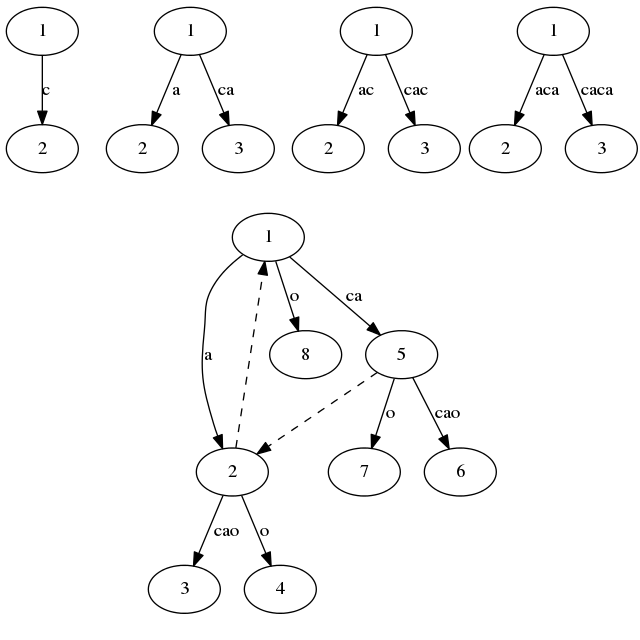
\includegraphics[width=1\textwidth]{media/cacao_vizualization.png}
	\caption{Izgradnja sufiksnog stabla za riječ cacao}
	\label{image:cacao}
\end{figure}

Na slici \ref{image:cacao} je prikazana izgradnja stabla za već klasičnu riječ cacao. Na ovim sufiksnim stablima čvor broj 1 uvijek predstavlja korijen stabla. Njegov roditelj nije prikazan jer se nikada ne mijenjaju veze iz ili prema tom čvoru.

Opis dodavanja svakog idućeg znaka iz riječi cacao.
\begin{enumerate}
	\item Prije dodavanja znakova. Aktivna točka je u korijenu stabla, a završna točka je u roditelj korijena.
	\item Dodavanje znaka c. Ne postoji ništa prije aktivne točke. U aktivnoj točki se dodaje znak c čime nastaje novi prijelaz i novi čvor. Sufkisna veza vodi do završne točke, te time završava dodavanje novih čvorova. Prijelazom iz završne točke znakom c nastaje nova aktivna točka -- korijen.
	\item Dodavanje znaka a. Svi čvorovi prije aktivne točke (listovi) dobivaju automatski znak a na kraj. U aktivnoj točki se dodaje prijelaz a te nastaje novi čvor označen brojem 2. Iduće stanje je roditelj od korijena no on već ima prijelaz za znak a te time ažuriranje stabla završava. Aktivna točka se dobiva prijelazom znakom a, a to je korijen stabla.
	\item Dodavanje znaka c. Svi čvorovi prije aktivne točke (listovi) dobivaju automatski znak c na kraj. U aktivnoj točki, tj. u korijenu već postoji prijelaz za znak c, što znači da je postupak ažuriranja stabla gotov. Nova aktivna točka postaje stanje do kojeg se dolazi koristeći znak c. To je stanje s oznakom (root, c), tj. nalazi se na bridu 1-3 iza slova c.
	\item Dodavanje znaka a. Svi čvorovi prije aktivne točke (listovi) dobivaju automatski znak a na kraj. U aktivnoj točki, tj. iza slova c na bridu 1-3 već postoji znak a što znači da je osvješavanje stabla završeno i da se aktivna točka samo pomiče koristeći znak a -- brid 1-3 iza ca (root, ca).
	\item Dodavanje znaka o. Svi čvorovi prije aktivne točke (listovi) dobivaju automatski znak o na kraj. U staroj aktivnoj točki, tj. iza slova ca na bridu 1-3 ne postoji znak o što znači da je potrebno dodati novu granu na tom mjestu. To se radi tako da se stvara novi čvor na tom mjestu, na slici čvor 5, te iz njega izlaze dva brida, jedan koji vodi do starog čvora (broj 6 na slici) i jedan koji vodi do novostvorenog čvora (broj 7 na slici). Sljedeće stanje u koje algoritam dolazi je (root, a). Dodavanjem znaka o se također mora razbiti brid te stvoriti novi čvor označen brojem 2, te iz njega izlaze dvije grane, jedna prema starom čvoru označenim brojem 3 i prema novom čvoru označeim brojem 4. Također dodaje se sufiksna veza iz prethodnog čvora označenog brojem 5 prema čvoru 2 jer je to stanje upravo sufiks prošlog stanja. Iduće stanje u koje algoritam dolazi je sufiks od (root, a), a to je (root, $\epsilon$). Iz njega ne postoji prijelaz za slovo o pa se stvara novi čvor označen brojem 8 te se stvara sufiksna veza iz prošlog čvora do trenutnog čvora, tj. iz čvora 2 do čvora 1. Nova aktivna točka je (root, $\epsilon$).
\end{enumerate}

\chapter{Rezultati testiranja}
	Za testiranje programske izvedbe \textit{Ukkonenovog} algoritma za izgradnju sufiksnog stabla koristili smo \textit{Bio-Linux 8} platformu koja se može preuzeti na \cite{biolinux}. 
	
\section{Postavljanje sustava}	
	\textit{Bio-Linux 8} je moćna, besplatna platforma prilagođena potrebama u bioinformatici koja se može instalirati na osobno računalo ili za to posebno predviđeni poslužitelj.  \textit{Bio-Linux 8} uključuje više of 250 bioinformatičkih paketa na bazni operacijski sustav \textit{GNU/Linux Ubuntu 14.04 LTS}.
	
	Međutim, naša programska izvedba \textit{Ukkonenovog} algoritma zahtijeva instalaciju dodatnog paketa koji je potreban za iscrtavanje sufiksnog stabla. Radi se o paketu \textit{graphviz} koji je moguće instalirati sljedećom naredbom
\begin{lstlisting}
sudo apt-get install libgraphviz-dev
\end{lstlisting}
	
\section{Izgradnja ostvarenog rješenja}
	Kako bi olakšali komajliranje ostvarenog programskog rješenja, koristili smo \textit{Makefile} datoteku. Ona omogućuje definiranje pravila kompajliranja izvornog teksta ostvarenog rješenja prema kojima se izgrađuju izvršne datoteke. Za potrebe ovog projekta izradili, kao rezultat izgradnje ostvarenog rješenja nastaju sljedeće izvršne datoteke:
\begin{itemize}
	\item trie - izvršna datoteka za izgradnju sufiksnog stobla
	\item test\_tree - izvršna datoteka koja provjerava ispravan rad izgradnje sufiksnog stabla
	\item visualize\_tree - izvršna datoteka koja prilikom izgradnje sufiksnog stabla, nakon svakog koraka, iscrtava trenutno stanje sufiksnog stabla
	\item create\_tests - izvršna datoteka koja čita genom u \textit{FASTA} formatu, te u zasebne datoteke sprema genome za potrebe testiranja
	\item test\_performance - izvršna datoteka koja čita testove koji se nalaze u zasebnim datotekama te prilikom izgradnje sufiksnog stabla mjeri utrošeno vrijeme i memoriju
\end{itemize}

\section{Escherichia Coli}
	Genom bakterije \textit{Escherichia Coli} preuzet je s \cite{ecoli}. 
	
	Nakon preuzimanja komprimirane datoteke i raspakiravanja iste, korištena je izvršna datoteke \textit{create\_tests} koja je kreirala zasebne datotke za testiranje u kazalu \textit{/tests/}. Izvršnom datotekom \textit{test\_performance} su zatim provedeni svi testovi te spremljeni rezultati izvođenja. Alatom \textit{gnuplot} su zatim iscrtane ovisnosti vremena izgradnje i memorije potrebne za izgradnju sufiksnog stabla u ovisnosti o veličini ulaznog niza.

\begin{figure}[h!]	
	\centering
	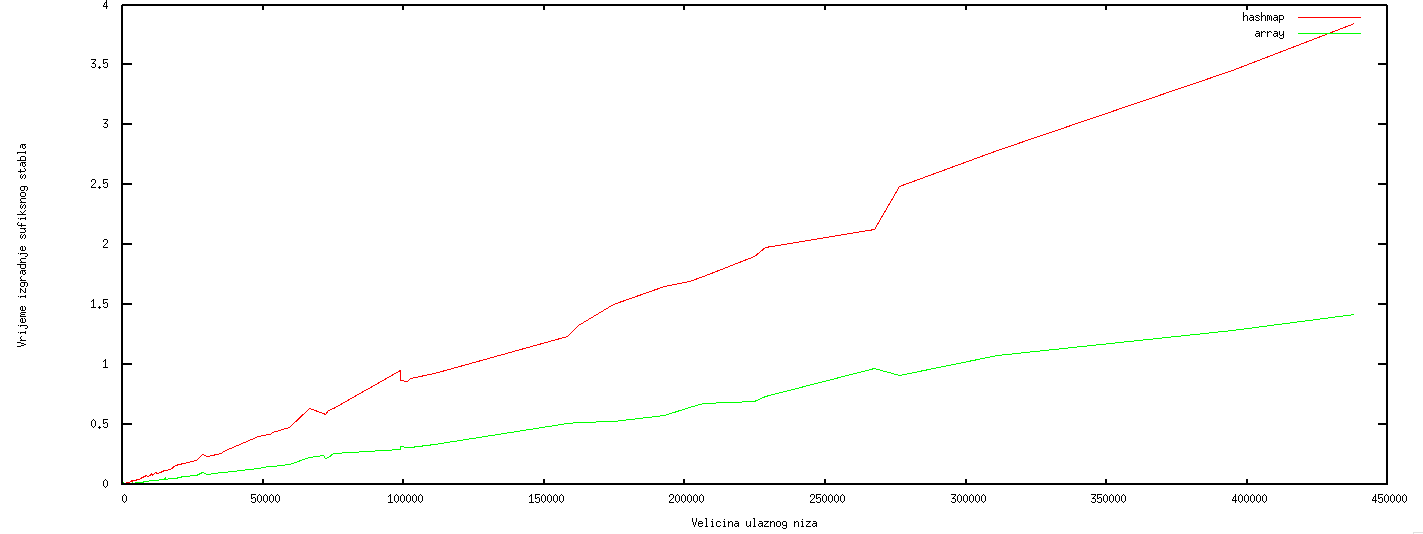
\includegraphics[width=1\textwidth]{media/time_1.png}
	\caption{Vremenska ovisnost o veličini ulaznog niza}
	\label{image:time}
\end{figure}

Na slici \ref{image:time} možemo vidjeti dva grafa. Crvenom je bojom označena vremenska ovisnost izgradnje sufiksnog stabla u slučaju kada ja kao struktura podataka čvora korištena \textit{hash} tablica dok je zelenom bojom označena vremenska ovisnost izgradnje sufiksnog stabla u slučaju kada ja kao struktura podataka čvora korišten \textit{niz}.

\pagebreak % to be sure the text below is not shown before this figure
\begin{figure}[h!]	
	\centering
	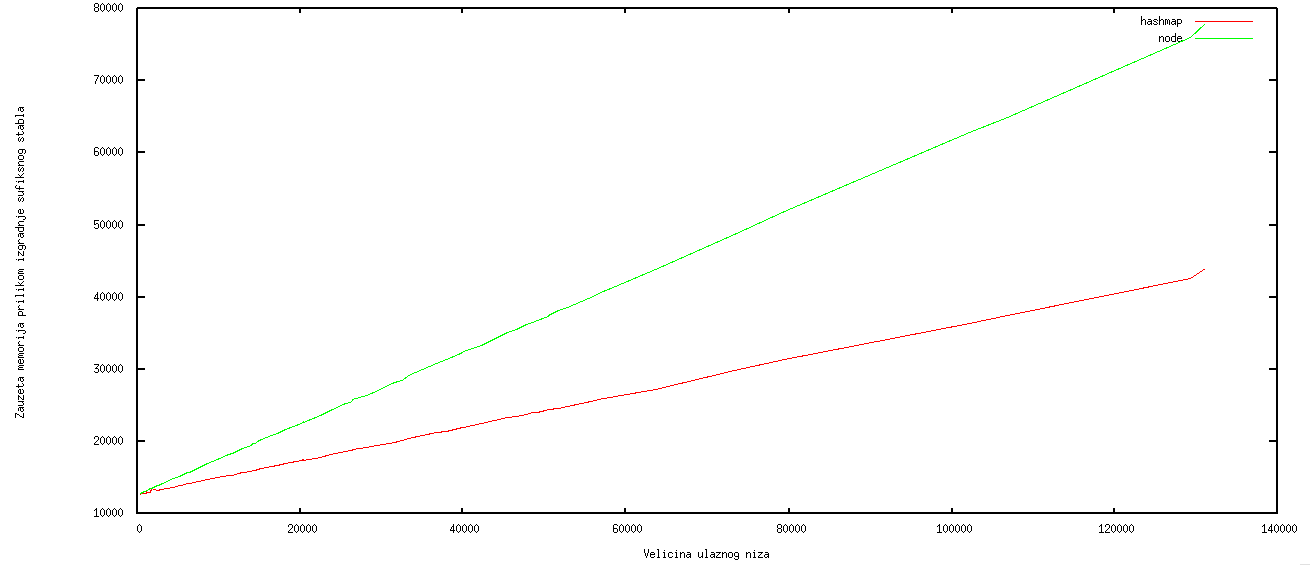
\includegraphics[width=1\textwidth]{media/memory_1.png}
	\caption{Memorijska ovisnost o veličini ulaznog niza}
	\label{image:memory}
\end{figure}

Slika \ref{image:memory} također koristi iste oznake kao i one za sliku \ref{image:time}. 

Na obje se slike može uočiti \textbf{linearan} porast vremena izvođenja, odnosno, potrebne memorije prilikom izgradnje sufiksnog stabla nad genomom bakterije \textit{Escherichia Coli}.


\section{Brochothrix Campestris}
	Genom bakterije \textit{Brochothrix Campestris} preuzet je s \cite{klamidija}. 
	
	U nastavku su prikazani rezultati performanse ostvarenog programskog rješenja nad genomom bakterije \textit{Brochothrix Campestris}.

\begin{figure}[h!]	
	\centering
	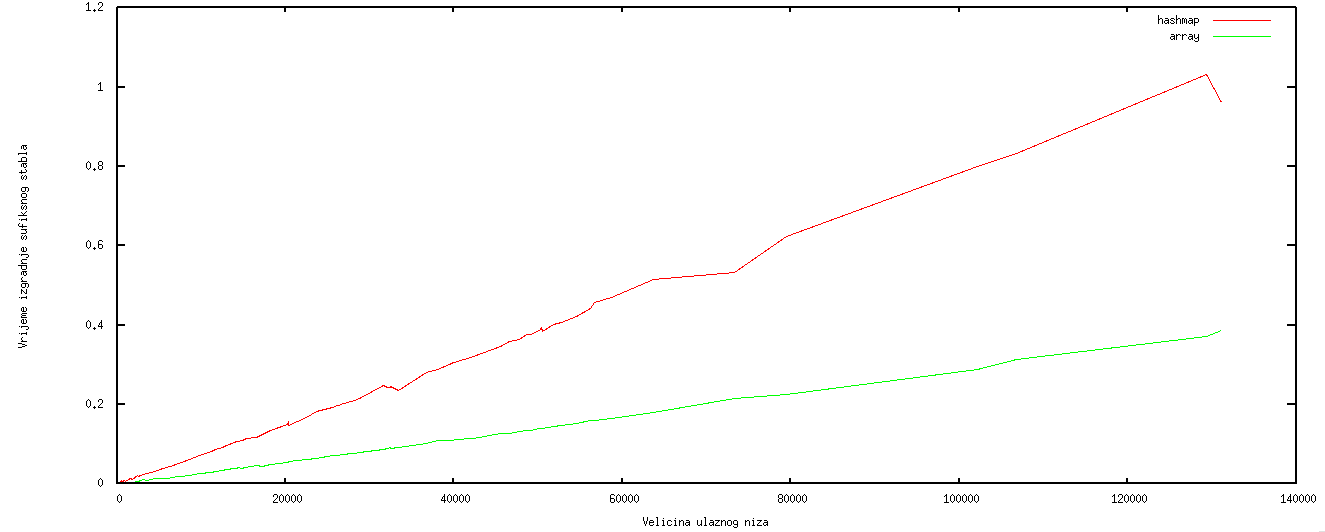
\includegraphics[width=1\textwidth]{media/time_2.png}
	\caption{Vremenska ovisnost o veličini ulaznog niza}
	\label{image:time1}
\end{figure}

\begin{figure}[h!]	
	\centering
	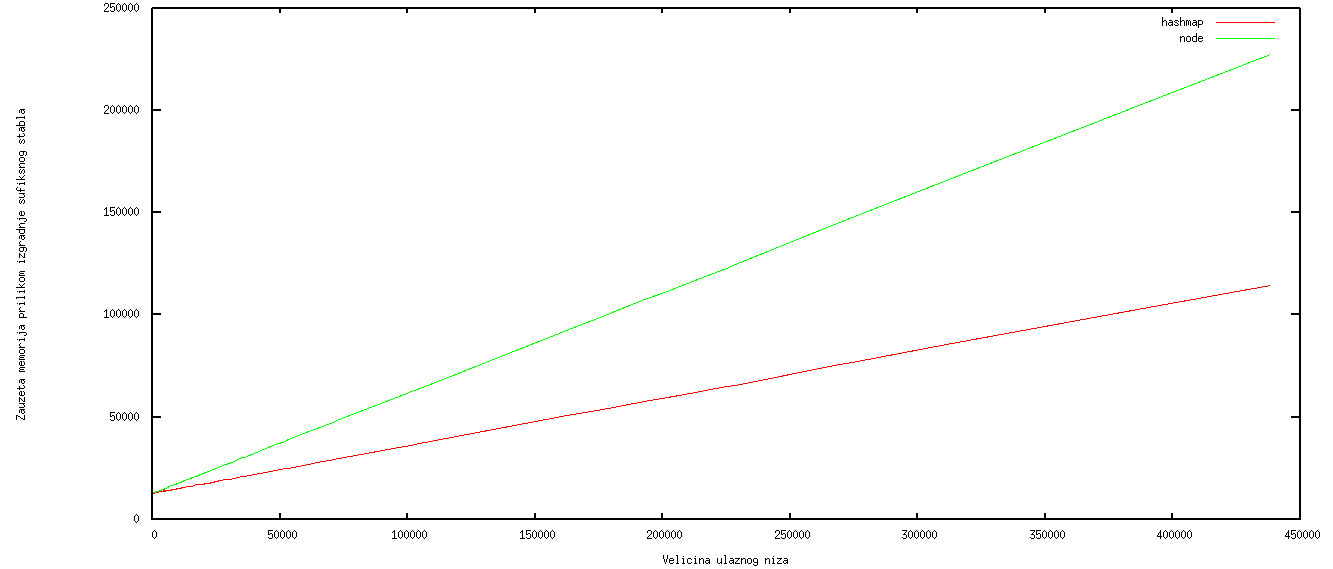
\includegraphics[width=1\textwidth]{media/memory_2.png}
	\caption{Memorijska ovisnost o veličini ulaznog niza}
	\label{image:memory1}
\end{figure}

\pagebreak

Na slici \ref{image:time1} te slici \ref{image:memory1}, možemo opet uočiti \textbf{linearan} porast vremena izvođenja, odnosno, potrebne memorije prilikom izgradnje sufiksnog stabla nad genomom bakterije \textit{Brochothrix Campestris}.

\chapter{Zaključak}
	\textit{Ukkonenov} algoritam za izgradnju sufiksnog stabla ima dvije prednosti. Prva je ta što je vremenska složenost izgradnje stabla linearna s obzirom na duljinu ulaznog niza znakova, tj. ako je $T$ ulazni niz znakova, onda je vremenska složenost \textit{Ukkonenovog} algortima $O(n)$ pri čemu je $n = |T|$.
	
	Druga prednost je što ima poželjno svojstvo procesiranja simbola s lijeva na desno te pritom ima izgrađeno sufiksno stablo za pročitani dio ulaznog niza, tj. ako smo pročitali prvih $k$ znakova ulaznog niza, $T = t_1 t_2 ... t_n$, nakon obrade simbola $t_k$, sufiksno stablo $STree(T^k)$ će biti u potpunosti izgrađeno.

 	Ostvareno programsko rješenje pokazuje da izgradnja sufiksnog stabla \textit{Ukkonenovim} algoritmom, i vremenski i memorijski, linearno ovisi o velicini ulaznog niza $T$.

\bibliography{literatura}
\bibliographystyle{fer}

\chapter{Sažetak}
Ukkonenov algoritam efikasno rješava problem izgradnje sufiksnog stabla. Vremenska i memorijska složenost je $O(n)$, tj. optimalna. Unatoč tome u praksi je memorijska konstanta često prevelika jer sufiksno stablo zauzima 10 do 50 puta više memorije nego li je veličina ulaznog niza. Zbog toga su su se dosta počela istraživati sufiksna polja koja zauzimaju puno manje memorije, a mogu u jednakoj složenosti odgovarati na skoro sve upite kao i sufiksna stabla.

Unatoč tome ovo je jedan od jednostavnijih efikasnih \textit{on-line} algoritama izgradnje sufiksnog stabla.

\end{document}
